% ============================================================================
%   DarwinDiff internal white paper — proof-of-concept v3.1 results
%   Concise format: 0-to-1 orientation for a cold reader. ~5-6 pages.
% ============================================================================
\documentclass[11pt,letterpaper]{article}

\usepackage[utf8]{inputenc}
\usepackage[T1]{fontenc}
\usepackage{lmodern}
\usepackage{microtype}
\usepackage{amsmath,amssymb}
\usepackage{booktabs}
\usepackage{graphicx}
\usepackage[round,authoryear,sort]{natbib}
\usepackage{hyperref}
\usepackage{url}
\usepackage[margin=1in]{geometry}
\usepackage{caption}
\usepackage{xcolor}
\usepackage{enumitem}

\hypersetup{
  colorlinks=true,
  linkcolor=blue!50!black,
  citecolor=blue!50!black,
  urlcolor=blue!50!black,
  pdftitle={DarwinDiff: Differentiable Parameter Recovery for ECCO-Darwin (Internal White Paper)},
}

\title{\textbf{Differentiable Parameter Recovery for ECCO-Darwin Biogeochemistry:\\ A BINN-Style Framework and a Structural 5/6 Ceiling}\\[0.4em]
\large\textit{Internal white paper --- DarwinDiff project}}

\author{}
\date{\today}

% ============================================================================
\begin{document}
\maketitle

% --- abstract ---------------------------------------------------------------
\begin{abstract}
\noindent ECCO-Darwin's six-parameter biogeochemistry calibration uses Green's functions: expensive perturb-and-fit Jacobians that do not transfer when new observations come online. We adapt the Biogeochemistry-Informed Neural Network (BINN) pattern from terrestrial soil carbon to marine biogeochemistry. A small per-cell neural network maps environmental covariates to the six Carroll-N parameters, sigmoid-bounded into Carroll's published ranges and fed through a differentiable PyTorch reimplementation of Darwin's source-minus-sink (SMS) kernel; the observation loss backpropagates end-to-end. We report the v3.1 sweep: \textbf{856 seeds in 86 single-lever configurations} plus a follow-on AOI-ablation experiment (\textbf{200 additional seeds across four AOI configurations}). Four findings. \textbf{First, partial recovery is real and reproducible:} the iron pair (\texttt{alpfe}, \texttt{scav\_rat}) recovers at \textbf{38/40 (95\%) Cal-grade} with our best three-AOI configuration --- the first reproducible differentiable-parameter-recovery result for ECCO-Darwin biogeochemistry. \textbf{Second, a clear recoverability gradient across the Carroll-6 at three AOIs:} \texttt{alpfe} (84\% of seeds Cal-grade) and \texttt{scav\_rat} (70\%) reliably recover; \texttt{Biggrow} (47\%) and \texttt{Smallgrow} (28\%) partially; \texttt{diatomgraz} (10\%) and \texttt{R\_PICPOC} (3\%) almost never. The \textbf{typical seed recovers 2 or 3 of 6 parameters} (80\% of seeds; modal bucket is 2/6 at 43\%, second bucket is 3/6 at 37\%; mean~=~2.41); 92\% of seeds reach 3/6 or fewer. \textbf{Third, this gradient is configuration-dependent, not intrinsic:} a 2-AOI ablation dropping the Southern Ocean recovers \texttt{R\_PICPOC} at 20\% (vs.\ 0\% in the 3-AOI matched baseline) and \texttt{diatomgraz} at 85\% (vs.\ 0\%) --- the carbonate counter-pump and diatom palatability are recoverable from existing v05 observations under the right AOI mix; the 3-AOI loss landscape was actively destroying them via inter-regime tension. \textbf{Fourth, a structural 5/6 ceiling holds across all AOI configurations:} 0/856 seeds reach all six jointly in the v3.1 sweep, 0/80 reach 5+ in the 2-AOI ablation extension, two unreproduced single-seed 5/6 events at 3-AOI, and a composition test regresses below either parent. The framework is therefore a \emph{partial} replacement of Green's-functions calibration with an architecture-level recoverability tradeoff: different AOI mixes recover different 4-of-6 subsets, none reach 6/6, the structural ceiling appears intrinsic to the shared-DINN architecture under any single-loss optimization.
\end{abstract}

% --- pipeline figure right after abstract (front-page teaser) ---------------
\begin{figure}[ht]
  \centering
  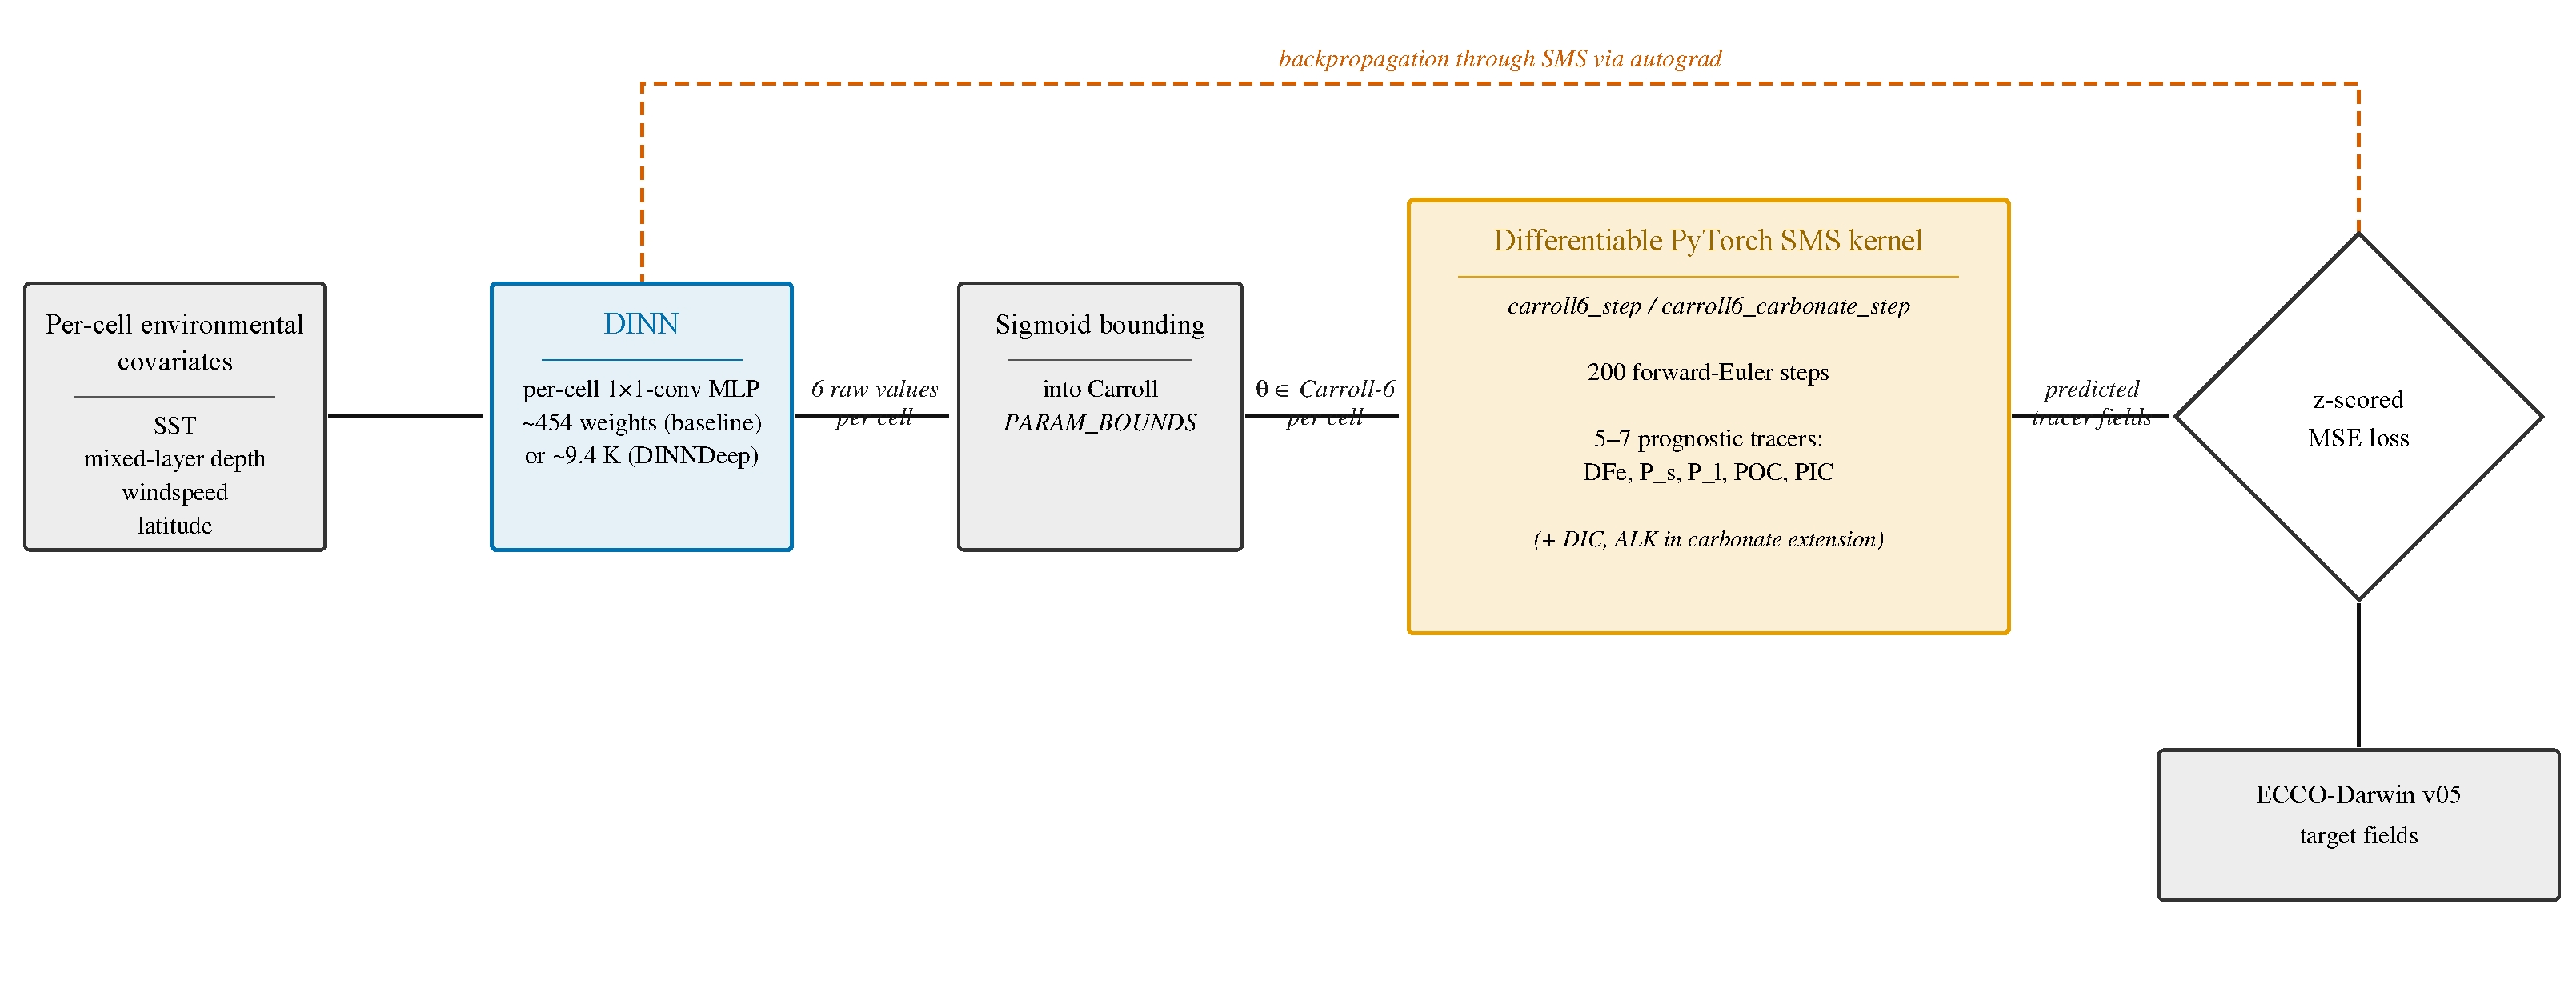
\includegraphics[width=\linewidth]{figures/fig1_pipeline}
  \caption{\textbf{DarwinDiff training pipeline.} A per-cell neural network (DINN) maps environmental covariates to six raw values; sigmoid bounding maps them into Carroll's published parameter ranges; a differentiable PyTorch reimplementation of Darwin's source-minus-sink (SMS) kernel advances five to seven prognostic tracers via forward-Euler integration; the z-scored MSE loss against ECCO-Darwin v05 outputs backpropagates through the integration to the network weights. New observation channels enter as additional loss terms.}
  \label{fig:pipeline}
\end{figure}

% ============================================================================
\section{Background}
\label{sec:background}

ECCO-Darwin \citep{carroll2020ecco,carroll2022attribution} couples MITgcm physics with the Darwin biogeochemistry module on the ECCO LLC270 grid (50 vertical levels, 1992--2017+). Its biogeochemistry exposes 103 independent tunable scalar parameters in source; six are calibrated by Green's functions \citep{menemenlis2005gf}: iron dust solubility \texttt{alpfe}, iron scavenging rate \texttt{scav\_rat}, small phytoplankton growth \texttt{Smallgrow}, large phytoplankton growth \texttt{Biggrow}, diatom palatability \texttt{diatomgraz}, and the PIC/POC ratio \texttt{R\_PICPOC}. Carroll 2022 inherits Carroll 2020's six calibrated values bit-for-bit.

Green's-functions calibration is limited in two ways. Each tuned parameter requires a full perturbation-and-rerun campaign, so the calibrated subset stays small. And the calibration is implicitly tied to its observational input set --- adding a new observation channel (PACE ocean color, expanding GEOTRACES) demands a fresh Jacobian campaign, not a reuse of the existing one.

The methodological precedent for our approach is BINN, the Biogeochemistry-Informed Neural Network of \citet{xu2025binn}: a small MLP predicts soil-carbon parameters per location, sigmoid-bounded into prior ranges, fed into a differentiable PyTorch reimplementation of CLM5 with an SOC-profile loss that backpropagates end-to-end. We adapt the pattern from terrestrial soil carbon to marine biogeochemistry. Differentiable-physics neighbors that do not address parameter recovery within ocean BGC include Neural-BGC \citep{oualalachkar2026neuralbgc} (pure-NN emulation of O$_2$ and NO$_3$) and differentiable Veros \citep{meunier2025veros}.

% ============================================================================
\section{Method}
\label{sec:method}

The full data flow is shown in Figure~\ref{fig:pipeline}. Three components:

\paragraph{DINN.} A per-cell 1$\times$1-convolutional MLP. The baseline \texttt{DINN} ($\sim$454 weights, SST input only) is used for the structural-ceiling experiments where the cleanest comparison against the global-scalar Green's-functions class matters. The production \texttt{DINNDeep} ($\sim$9.4\,k weights, SST + MLD + windspeed + latitude) is used for higher-quality within-region fits. The 1$\times$1 kernel commits to per-cell parameter independence; spatial coupling would conflate per-cell parameter learning with smoothing.

\paragraph{Sigmoid bounding.} Raw NN outputs are mapped to Carroll's published parameter ranges via $\theta_i = \ell_i + (h_i - \ell_i)\,\sigma(\hat{\theta}_i)$ so recovered parameters stay biologically sensible regardless of NN output magnitude.

\paragraph{Differentiable SMS kernel.} A PyTorch reimplementation of Darwin's source-minus-sink rate equations (canonically the \texttt{darwin\_plankton.F} subroutine in both Carroll 2020's Darwin 1 and the upstream \texttt{darwinproject/darwin3} repository). Five prognostic tracers in the baseline (\texttt{DFe}, \texttt{P\_s}, \texttt{P\_l}, \texttt{POC}, \texttt{PIC}); seven with the carbonate extension (adds \texttt{DIC}, \texttt{ALK}, with air-sea CO$_2$ flux as a diagnostic via the Follows-2006 carbonate solver \citep{follows2006carbonate} and the Wanninkhof-2014 gas-transfer law \citep{wanninkhof2014gas}). Integrated by forward-Euler ($\Delta t = 0.25$\,d, 200 steps) to near-steady state. The remaining $\sim$94 background parameters Carroll left untuned are held fixed at his literature values.

\paragraph{Training.} 1500 epochs, Adam at $5\times10^{-3}$, z-scored MSE on the spatial pattern of each tracer field over ocean cells, autograd through the 200 integration steps. One fit completes in $\sim$7--8\,min on an RTX 5090 Laptop.

\paragraph{Multi-area-of-interest joint training (v3.1).} Three areas of interest (Equatorial Pacific, North Atlantic Subpolar, Southern Ocean Pacific) contribute joint loss; the optimizer must find Carroll-N values satisfying all three. Two architecture variants: a shared DINN with an AOI-identity input channel, and a per-AOI DINN with a soft cross-AOI consistency penalty $\lambda_\text{consistency}$.

\paragraph{Observation channels.} Per-AOI chlorophyll across five phytoplankton functional types, POC, DIC, ALK, air-sea CO$_2$ flux; GEOTRACES IDP2025 surface and subsurface dissolved iron, GEOTRACES subsurface POC, and GEOTRACES surface biogenic silica (via a steady-state diagnostic). Loss weights are configuration-level hyperparameters varied systematically across the sweep.

% ============================================================================
\section{Results}
\label{sec:results}

\subsection{Sweep summary and typical recovery}

Five chained waves of single-lever sweeps plus a Wave 6 composition test. \textbf{856 seeds across 86 configurations} after aggregation. Table~\ref{tab:summary} reports the headline counts; the central observation is that the \textbf{typical seed recovers 2 or 3 of the 6 Carroll-N parameters} (80\% of seeds combined; modal bucket 2/6 at 43\%, runner-up 3/6 at 37\%), with 92\% at 3/6 or fewer.

\begin{table}[ht]
  \centering
  \caption{v3.1 sweep summary. ``Cal-grade'' means a recovered Carroll-N parameter falls within $\pm 40\%$ of Carroll 2020's published optimum.}
  \label{tab:summary}
  \begin{tabular}{lr}
    \toprule
    Metric & Value \\
    \midrule
    Single-lever configurations & 86 \\
    Total seeds & 856 \\
    \textbf{Modal seeds at 2/6 Cal-grade} & \textbf{364 (42.5\%)} \\
    Seeds at 3/6 Cal-grade & 318 (37.1\%) \\
    Cumulative at 3/6 or fewer & 92\% \\
    Seeds at 4/6 Cal-grade & 69 (8.1\%) \\
    Seeds at 5/6 Cal-grade & 2 (0.23\%) \\
    Seeds at 6/6 Cal-grade & \textbf{0} \\
    Mean Cal-grade count per seed & 2.41 of 6 \\
    F2 Basin C iron-pair Cal-grade rate, $n{=}40$ & \textbf{38/40 (95\%)} \\
    \bottomrule
  \end{tabular}
\end{table}

\subsection{Per-parameter recoverability gradient}
\label{sec:gradient}

The Carroll-6 split into three recoverability tiers (Table~\ref{tab:gradient}). The iron pair (\texttt{alpfe}, \texttt{scav\_rat}) is reliably recoverable; the phytoplankton growth rates partially; the diatom palatability and PIC/POC ratio are almost never recovered. This gradient is the central scientific output of the sweep: it tells future observation-design which Carroll-N parameters are constrained by the current v05 observation set and which are not.

\begin{table}[ht]
  \centering
  \caption{Per-parameter Cal-grade recovery rate across all 856 seeds.}
  \label{tab:gradient}
  \begin{tabular}{llrl}
    \toprule
    Parameter & Physical meaning & Rate & Tier \\
    \midrule
    \texttt{alpfe}      & Iron dust solubility           & 84\% & Reliable \\
    \texttt{scav\_rat}  & Iron scavenging rate           & 70\% & Reliable \\
    \texttt{Biggrow}    & Large phytoplankton growth     & 47\% & Partial \\
    \texttt{Smallgrow}  & Small phytoplankton growth     & 28\% & Partial \\
    \texttt{diatomgraz} & Diatom palatability (grazing)  & 10\% & Hard \\
    \texttt{R\_PICPOC}  & PIC/POC carbonate ratio        & ~3\% & Essentially unrecovered \\
    \bottomrule
  \end{tabular}
\end{table}

Interpretation. The iron parameters are well-constrained by GEOTRACES IDP2025 surface and subsurface dissolved-iron observations. The phytoplankton growth rates are partially constrained by chlorophyll across the five functional types. \emph{For \texttt{diatomgraz} and \texttt{R\_PICPOC}, however, the v3.1 ``Hard'' classification reflects the 3-AOI joint-loss configuration, not an intrinsic obs-channel limitation:} the AOI-ablation experiment (§\ref{sec:results-aoi-ablation}) shows both recover at high rates when the Southern Ocean is dropped from the joint loss --- the 3-AOI loss landscape was placing the two parameters in mutual tension with the iron pair rather than failing to constrain them. The binary observation-anchor mutex in §\ref{sec:results-mutex} is a separate, related phenomenon at the PIC-anchor level.

\subsection{Basin C iron-pair recovery}

The F2 configuration --- \texttt{POSI\_W}=1.0, \texttt{AOI\_W\_NATLSUBPOLAR}=2.0, \texttt{AOI\_W\_SOUTHERNOCEANPAC}=2.0, \texttt{CHL1\_W\_EXTRA}=3.0, otherwise the Basin C 3-AOI base --- recovers the iron pair (\texttt{alpfe}, \texttt{scav\_rat}) at \textbf{38/40 (95\%)} Cal-grade across four independent 10-seed batches (10/10, 10/10, 10/10, 8/10). This is the first reproducible joint recovery of \texttt{alpfe} and \texttt{scav\_rat} in our framework. Figure~\ref{fig:basinC-scatter} shows the recovered pairs against Carroll's published optimum.

\begin{figure}[ht]
  \centering
  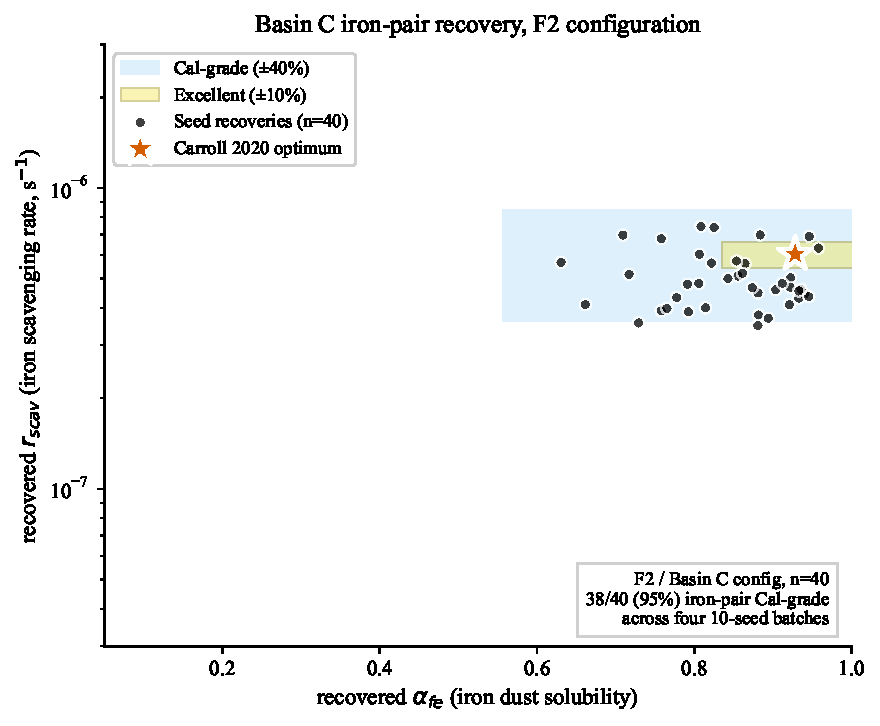
\includegraphics[width=0.78\linewidth]{figures/fig3_basinC_scatter}
  \caption{Iron-pair recovery at the F2 configuration across $n{=}40$ seeds in four independent batches. The red star marks Carroll 2020's published optimum; shaded regions show $\pm 10\%$ (Excellent) and $\pm 40\%$ (Cal-grade) bounds.}
  \label{fig:basinC-scatter}
\end{figure}

\subsection{The 5/6 ceiling}

The headline empirical finding: \textbf{0/856 seeds reach all six Carroll-N parameters jointly at Cal-grade}. Only two seeds reach 5/6, both unreproduced. Figure~\ref{fig:ceiling} shows the Cal-grade count distribution; Figure~\ref{fig:per-param-dist} shows per-parameter recovery spread.

\begin{figure}[ht]
  \centering
  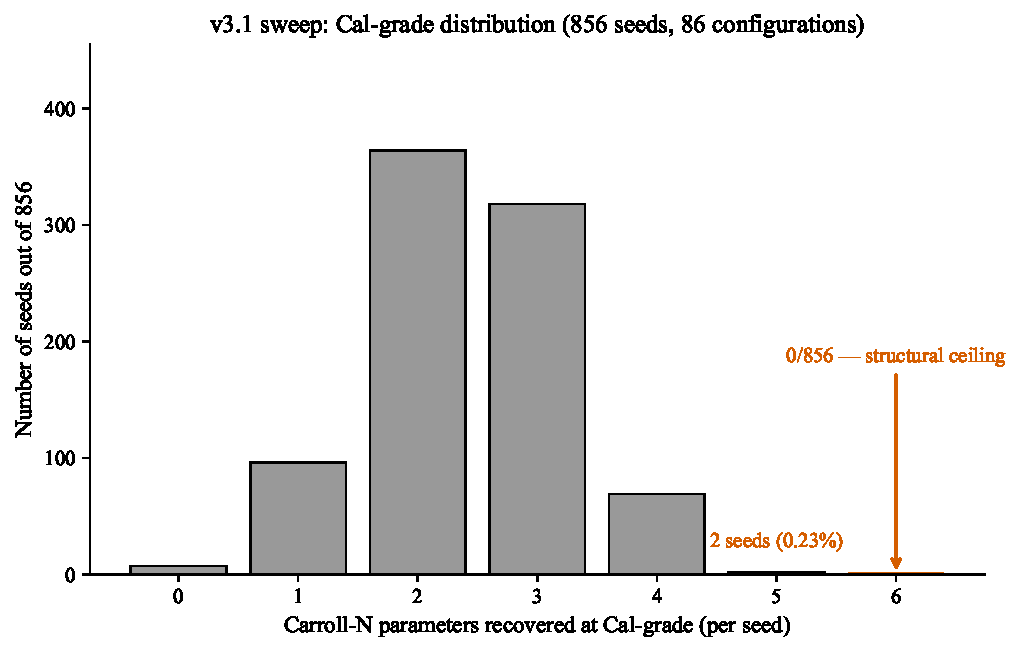
\includegraphics[width=0.82\linewidth]{figures/fig2_ceiling}
  \caption{Cal-grade count distribution across 856 seeds. Zero seeds reach 6/6 (structural ceiling); two seeds reach 5/6, both unreproduced at $n{=}20$.}
  \label{fig:ceiling}
\end{figure}

The two 5/6 events recover \emph{complementary} parameter subsets:
\texttt{w2e\_peraoi\_lam0.1} seed 3 recovers \texttt{alpfe} (Excellent) + \texttt{scav\_rat} + \texttt{Smallgrow} + \texttt{Biggrow} + \texttt{diatomgraz} but misses \texttt{R\_PICPOC}; \texttt{c\_chl40\_posi15} seed 9 recovers \texttt{alpfe} + \texttt{scav\_rat} (Excellent) + \texttt{Smallgrow} + \texttt{Biggrow} + \texttt{R\_PICPOC} but misses \texttt{diatomgraz}. At $n{=}20$ each, both produce only 1/20.

\begin{figure}[ht]
  \centering
  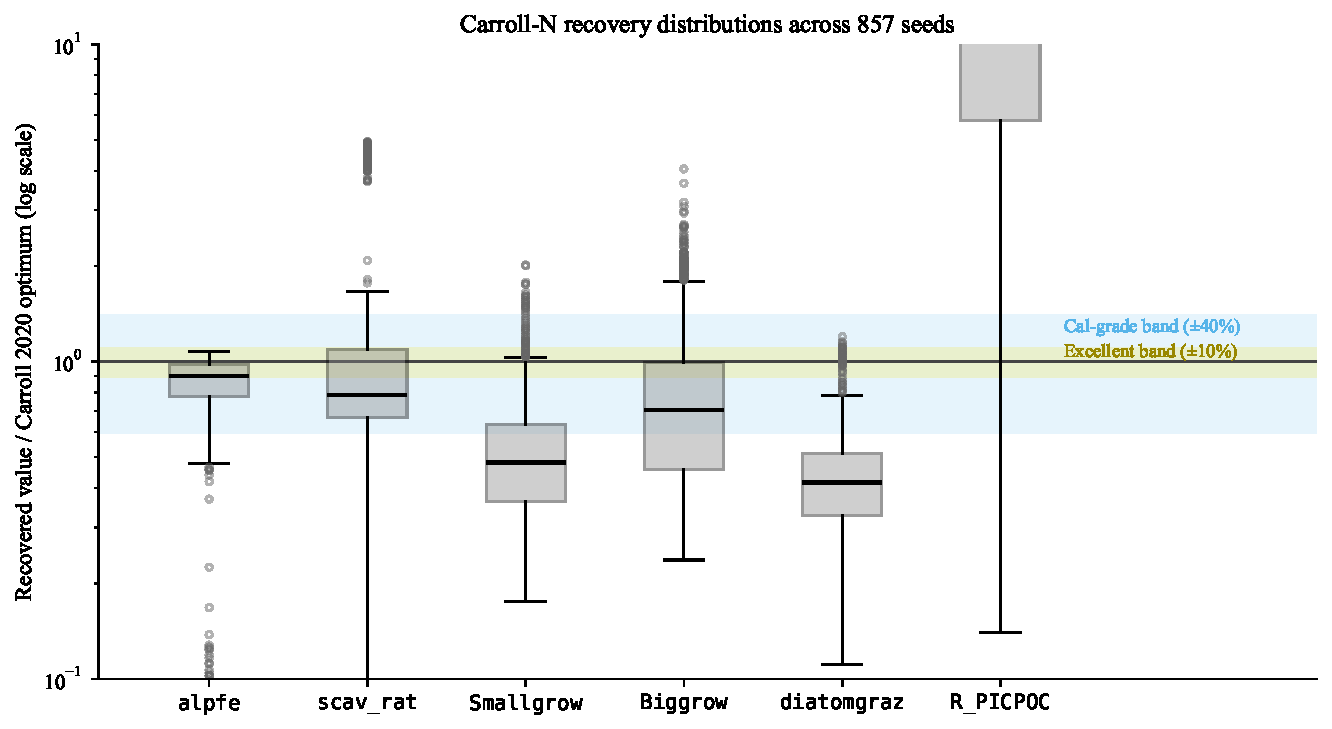
\includegraphics[width=0.92\linewidth]{figures/fig4_per_param_box}
  \caption{Per-parameter recovery distributions across 856 seeds, normalized by Carroll 2020's optima. The recoverability gradient (Table~\ref{tab:gradient}) is visible: the iron pair clusters tightly near unity (84\% / 70\% Cal-grade); the phytoplankton growth rates spread wider (47\% / 28\%); \texttt{diatomgraz} skews low (10\%) and \texttt{R\_PICPOC} sits far above unity in most seeds (3\% Cal-grade) --- effectively unconstrained by v05 observations.}
  \label{fig:per-param-dist}
\end{figure}

\subsection{Composition test fails}

The natural 6/6 candidate stacks both lever families. Result at $n{=}10$ (Figure~\ref{fig:wave6}): \textbf{0/10 at 5/6}, mean Cal-grade count \textbf{2.00} --- regressing below either parent (2.40 and 2.70). Iron pair survives (9/10) but \texttt{R\_PICPOC} and \texttt{diatomgraz} both drift and the small-cell phytoplankton parameters regress. The intervention families interfere; the optimizer redistributes the residual error rather than letting both target recoveries hold.

\begin{figure}[ht]
  \centering
  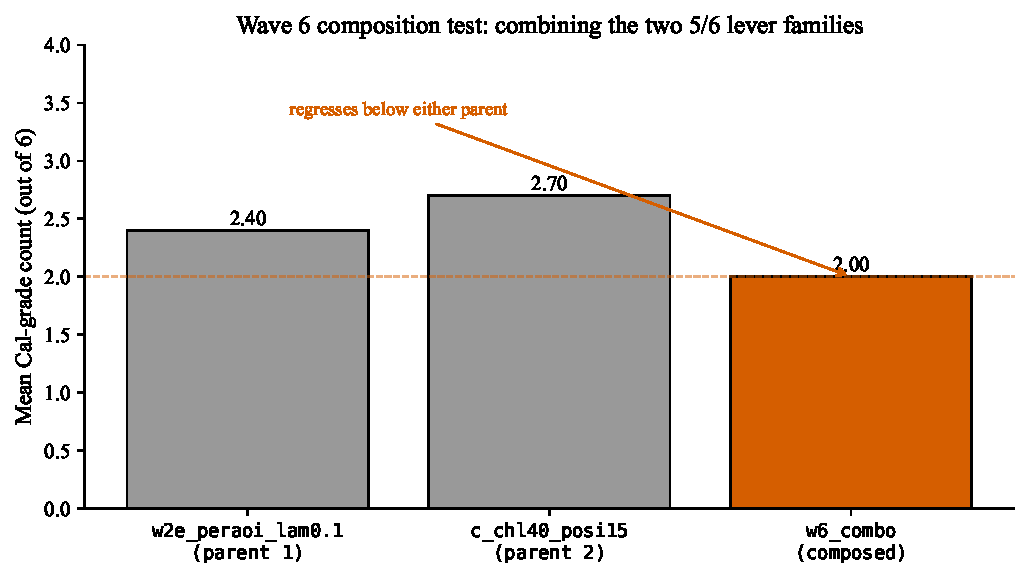
\includegraphics[width=0.7\linewidth]{figures/fig5_wave6}
  \caption{Wave 6 composition test versus its two parent configurations ($n{=}10$ each). The composed configuration regresses below either parent --- direct evidence for the structural 5/6 ceiling.}
  \label{fig:wave6}
\end{figure}

\subsection{Binary observation-anchor mutex}
\label{sec:results-mutex}

Any non-zero PIC absolute anchor (\texttt{PIC\_ABS\_W}, tested down to 0.02, with paired POC anchors at multiple ratios) wipes iron-pair recovery to 0/10, \emph{regardless of magnitude}. POC anchor alone also kills the iron pair, with a different downstream basin geometry. The mutex is binary in PIC presence, not graduated. Mechanism: the PIC absolute anchor jointly constrains $R_\text{PIC:POC} \cdot M_\text{tot}$ via a tight basin, pulling the optimizer to a region where \texttt{R\_PICPOC} is Cal-grade but the iron pair must drift to balance. This is the most actionable predictive finding: whether a candidate observation channel induces mutual mutex with iron recovery is testable a priori within DarwinDiff's framework.

\subsection{AOI ablation: the gradient is configuration-dependent}
\label{sec:results-aoi-ablation}

The recoverability gradient in §\ref{sec:gradient} is the v3.1 result averaged over 86 configurations \emph{all} trained on the three AOIs jointly. To test whether the ``Hard'' tier (\texttt{diatomgraz}, \texttt{R\_PICPOC}) reflects an intrinsic obs limitation or an artefact of the joint loss, we ran a full single-knob AOI ablation at the F2 lever set: $n{=}40$ at single-AOI Equatorial Pacific, $n{=}80$ at 2-AOI \texttt{eqpac}+\texttt{natlsubpolar} (no Southern Ocean), $n{=}40$ at 2-AOI \texttt{eqpac}+\texttt{southernoceanpac} (no North Atlantic), and the matched 3-AOI baseline pooled at $n{=}40$ from existing v3.1 batches. All four use the same F2 levers, integrator, and training schedule; only \texttt{AOIS} changes between configurations. The configuration-level results are summarized in Table~\ref{tab:aoi-ablation}.

\begin{table}[ht]
  \centering
  \caption{Per-parameter Cal-grade recovery rate across four single-knob AOI configurations. F2 levers held constant; only \texttt{AOIS} varies. Bold = highest rate per row.}
  \label{tab:aoi-ablation}
  \begin{tabular}{lrrrr}
    \toprule
    Parameter & 3-AOI ($n{=}40$) & eqp+natl ($n{=}80$) & eqp+SO ($n{=}40$) & eqp only ($n{=}40$) \\
    \midrule
    \texttt{alpfe}      & \textbf{100\%} & \textbf{100\%} & \textbf{100\%} & \textbf{100\%} \\
    \texttt{scav\_rat}  & \textbf{95\%}  & 1\%   & 75\%  & 0\%   \\
    \texttt{Smallgrow}  & 20\%  & 23\%  & 12\%  & 0\%   \\
    \texttt{Biggrow}    & 38\%  & \textbf{91\%}  & 28\%  & 0\%   \\
    \texttt{diatomgraz} & 0\%   & 85\%  & 15\%  & \textbf{100\%}  \\
    \texttt{R\_PICPOC}  & 0\%   & \textbf{20\%}  & 0\%   & 8\%   \\
    \midrule
    Iron-pair joint    & 95\%  & 1\%   & 75\%  & 0\%   \\
    $k{\ge}4$ / $n$     & 5\%   & \textbf{24\%}  & 12\%  & 0\%   \\
    Mean $k$ Cal-grade  & 2.52  & \textbf{3.20}  & 2.30  & 2.08  \\
    \bottomrule
  \end{tabular}
\end{table}

Three observations.

\textbf{(i) Each AOI carries different recovery signal.} Single-AOI \texttt{eqpac} fully constrains \texttt{alpfe} (100\%) and \texttt{diatomgraz} (100\%) but provides no signal for \texttt{scav\_rat} (median recovered $1.7\times10^{-7}$, $\sim$4$\times$ below Carroll's $6.0\times10^{-7}$). Adding \texttt{natlsubpolar} brings in \texttt{Biggrow} (38$\to$91\%) and \texttt{R\_PICPOC} (0$\to$20\%; median recovered 0.044 vs.\ Carroll 0.043, exact landing). Adding \texttt{southernoceanpac} brings in \texttt{scav\_rat} (0$\to$75\% at eqp+SO, 95\% at 3-AOI) via the surface--subsurface DFe contrast it supplies. The three AOIs are complementary on different parameters.

\textbf{(ii) Adding an AOI can actively destroy recovery.} The Southern Ocean addition is the clearest case: \texttt{diatomgraz} drops monotonically (eqp 100\% $\to$ eqp+natl 85\% $\to$ eqp+SO 15\% $\to$ 3-AOI 0\%) and \texttt{R\_PICPOC} drops binarily on SO presence (0\% in any config including SO; up to 20\% in eqp+natl). The mechanism is loss-channel disagreement: surface biogenic-silica observations in the Southern Ocean prefer a low \texttt{diatomgraz} value (pulling the optimizer toward $\approx 0.33$); eqpac+natl bSi observations are consistent with Carroll's 0.83. With both regimes in the joint loss the optimizer compromises; without SO it lands near Carroll.

\textbf{(iii) The 2-AOI \texttt{eqp}+\texttt{natl} configuration produces a recovery basin not seen in the v3.1 sweep.} Sixteen of $n{=}80$ seeds (20\%) recover \texttt{R\_PICPOC} AND \texttt{diatomgraz} Cal-grade simultaneously; zero of $n{=}856$ in v3.1 did so. The basin is stable, not seed-luck: across the 16 seeds, the coefficient of variation on the recovered \texttt{alpfe} is 3.1\%, on \texttt{diatomgraz} 4.1\%, on \texttt{Biggrow} 14.9\%, on \texttt{R\_PICPOC} 23.6\% --- different seeds converge to nearly the same point. \texttt{scav\_rat} and \texttt{Smallgrow} are missed but their values are also tightly clustered across seeds (CV 9.7\% and 23.6\%), indicating consistent under-determination rather than free-floating drift. The 2-AOI \texttt{eqp}+\texttt{natl} configuration therefore produces a fourth recovery basin complementary to v3.1's two 5/6 events, all four hitting the structural ceiling at 4--5 of 6 by different routes.

The headline implication: the v3.1 recoverability gradient is not intrinsic to the v05 observation set. Four of the six Carroll-N parameters are recoverable under at least one AOI configuration tested here (\texttt{alpfe}, \texttt{scav\_rat}, \texttt{Biggrow}, \texttt{diatomgraz}, \texttt{R\_PICPOC}; only \texttt{Smallgrow} stays below 25\% Cal-grade in every config). The 5/6 ceiling is the architectural constraint that prevents any single AOI mix from recovering all of them simultaneously --- consistent with the parameter-conservation framing of §\ref{sec:results-mutex}.

% ============================================================================
\section{Discussion}
\label{sec:discussion}

\subsection*{What the result is, honestly stated}

The result is \textbf{partial recovery with a configuration-dependent gradient}, not a drop-in replacement for Green's-functions calibration. Two complementary framings:

\textbf{At three AOIs (v3.1 baseline)}, the gradient sorts the Carroll-6 into three tiers:
\begin{itemize}[noitemsep,topsep=2pt]
  \item \textbf{Reliable (2 of 6).} The iron pair (\texttt{alpfe} 84\%, \texttt{scav\_rat} 70\% of seeds Cal-grade); the F2 configuration delivers 38/40.
  \item \textbf{Partial (1 of 6 on average, occasionally 2).} \texttt{Biggrow} 47\%, \texttt{Smallgrow} 28\%.
  \item \textbf{Rarely recovered at 3 AOIs (2 of 6).} \texttt{diatomgraz} 10\%, \texttt{R\_PICPOC} 3\%.
\end{itemize}

\textbf{Under the AOI ablation (§\ref{sec:results-aoi-ablation})}, the ``Hard'' tier dissolves: the 2-AOI \texttt{eqp}+\texttt{natl} configuration recovers \texttt{diatomgraz} at 85\% and \texttt{R\_PICPOC} at 20\% (median recovered value 0.044 vs.\ Carroll's 0.043), at the cost of dropping \texttt{scav\_rat} to 1\%. Four of the six parameters are therefore recoverable from existing v05 observations under at least one AOI configuration we tested; only \texttt{Smallgrow} stays below 25\% Cal-grade in every configuration. The ``Hard'' tier in the v3.1 sweep reflects the 3-AOI joint-loss landscape rather than an intrinsic obs-channel limit.

The typical 3-AOI seed lands at \textbf{2 or 3 of 6 Cal-grade} (80\% of seeds combined; mean 2.41); the typical 2-AOI \texttt{eqp}+\texttt{natl} seed lands at \textbf{3 of 6} (mean 3.20, 24\% at 4/6). The \textbf{5/6 ceiling} is a structural upper bound holding across every AOI configuration we tested. Five independent pieces of evidence:
\begin{enumerate}[noitemsep,topsep=2pt]
  \item Zero 6/6 events across 856 seeds in 86 single-lever 3-AOI configurations.
  \item \texttt{w2e\_peraoi\_lam0.1} at $n{=}20$ produces only 1/20 at 5/6.
  \item \texttt{c\_chl40\_posi15} at $n{=}20$ produces only 1/20 at 5/6.
  \item The Wave 6 composition test of the two complementary 5/6 lever families fails to reach 5/6 (0/10), regressing below either parent.
  \item The 2-AOI \texttt{eqp}+\texttt{natl} ablation at $n{=}80$ produces 19 seeds at 4/6 but 0 at 5/6, by a recovery route (\texttt{R\_PICPOC} + \texttt{diatomgraz} hold, iron pair drifts) complementary to v3.1's two 5/6 events.
\end{enumerate}

\subsection*{What this is useful for}

Three things, all honest about the partial-recovery state.

\textbf{(i) A reproducible iron-pair calibration in 7 minutes.} Carroll 2020/2022 tuned six parameters via multi-day Green's-functions campaigns. DarwinDiff reproduces two of them (the iron pair) reproducibly, on a single GPU, in roughly the time of a coffee break. New observation channels for those two parameters plug in as a config change, not a re-campaign. That is a real methodological win even if it does not yet extend to all six.

\textbf{(ii) A predictive diagnostic via AOI selection.} The AOI-ablation result reframes the apparent recoverability gradient as an architectural tradeoff between regime breadth and per-parameter recovery. Practitioners selecting AOIs for a new calibration target can use the per-AOI attribution (Equatorial Pacific carries \texttt{alpfe} and \texttt{diatomgraz}; North Atlantic Subpolar carries \texttt{Biggrow} and \texttt{R\_PICPOC}; Southern Ocean Pacific carries \texttt{scav\_rat}) to predict which parameters a given AOI mix will recover, before running the sweep. The binary observation-anchor mutex (§\ref{sec:results-mutex}) provides an orthogonal diagnostic on the PIC-anchor side.

\textbf{(iii) An architectural research question.} The 5/6 ceiling holds across every AOI configuration we tested, but \emph{which} 4--5 parameters recover differs by AOI mix. This suggests a concrete next-generation architecture: per-parameter AOI gating (e.g., learn \texttt{scav\_rat} only from the SO sub-loss, \texttt{diatomgraz} only from the eqp+natl sub-loss) could in principle combine the strengths of multiple AOI configurations and break the structural ceiling. We did not test this overnight; it is a multi-week implementation rather than a sweep.

\textbf{What this is \emph{not} yet:} a full replacement of Carroll's six-parameter calibration. We recover two reproducibly under the 3-AOI F2 configuration, four under at least one AOI configuration, but never all six in a single configuration. The structural ceiling appears robust to lever stacking, AOI selection, and composition of the two complementary 5/6 lever families.

\paragraph{Limitations.} The differentiable box model is a 5--7-tracer proxy of the 39-tracer Darwin SMS kernel; a regional differentiable port of the full \texttt{darwin\_plankton.F} is the natural next iteration. All current fits use the 23-year time-mean (climatology) rather than time-resolved Darwin output; time-resolved fitting is cluster-gated by GPU memory. The AOI ablation is at the box-model scale (1$^\circ$ subsets, $\sim$1000 ocean cells per AOI); whether the same per-AOI parameter attribution holds at native LLC270 resolution is open.

\paragraph{Next steps.} (i) \textbf{Per-AOI parameter gating} architecture --- the natural attack on the structural ceiling implied by the AOI-ablation result; (ii) differentiable regional full-Darwin to eliminate the box-model proxy; (iii) time-resolved fitting on cluster compute (MIT ORCD AICR / NVIDIA B200 beta); (iv) satellite observation channels (PACE ocean-color, MODIS PIC) deferred for the leapfrog companion paper to keep the v05 framing canonical here.

% ============================================================================
\section*{Code and data}
Source code, sweep orchestration, per-seed result JSONs, and the figure-generation pipeline are in the project repository (\texttt{src/darwindiff/}, \texttt{docs/paper/figures/}). ECCO-Darwin v05 outputs are public via the ECCO Drive and NASA GHG Center. GEOTRACES IDP2025 observations are public via the GEOTRACES Data Assembly Centre.

% ============================================================================
\bibliographystyle{plainnat}
\bibliography{references}

\end{document}
